\documentclass{standalone}
\usepackage{pgfplots}
\pgfplotsset{compat=1.18}
\usepgfplotslibrary{fillbetween}

\begin{document}
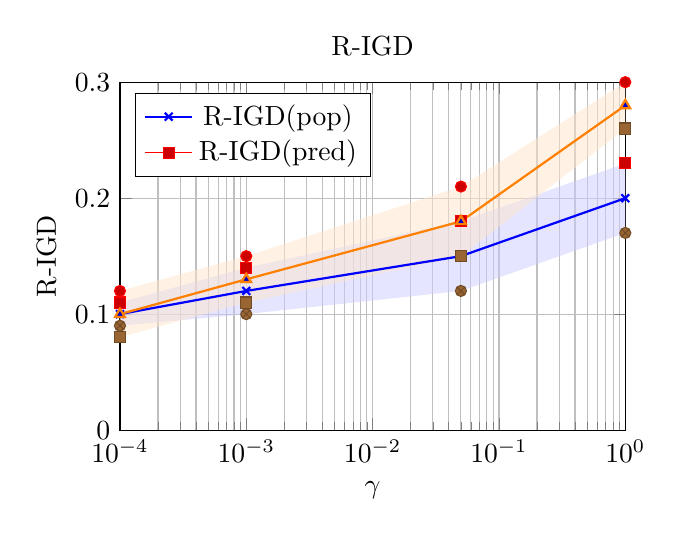
\begin{tikzpicture}
\begin{axis}[
    width=8cm, height=6cm,
    xlabel={$\gamma$},
    ylabel={R-IGD},
    xmin=1e-04, xmax=1e+00,
    ymin=0.0, ymax=0.3,
    xmode=log,
    legend pos=north west,
    grid=both,
    title={R-IGD}
]

% Data for R-IGD(pop)
\addplot+[blue, mark=x, thick] plot coordinates {
    (1e-04, 0.1)
    (1e-03, 0.12)
    (5e-02, 0.15)
    (1e+00, 0.2)
};

% Shaded area for R-IGD(pop)
\addplot+[name path=pop_upper, draw=none] coordinates {
    (1e-04, 0.11)
    (1e-03, 0.14)
    (5e-02, 0.18)
    (1e+00, 0.23)
};
\addplot+[name path=pop_lower, draw=none] coordinates {
    (1e-04, 0.09)
    (1e-03, 0.10)
    (5e-02, 0.12)
    (1e+00, 0.17)
};
\addplot[blue!20, opacity=0.5] fill between[of=pop_upper and pop_lower];

% Data for R-IGD(pred)
\addplot+[orange, mark=triangle*, thick] plot coordinates {
    (1e-04, 0.1)
    (1e-03, 0.13)
    (5e-02, 0.18)
    (1e+00, 0.28)
};

% Shaded area for R-IGD(pred)
\addplot+[name path=pred_upper, draw=none] coordinates {
    (1e-04, 0.12)
    (1e-03, 0.15)
    (5e-02, 0.21)
    (1e+00, 0.3)
};
\addplot+[name path=pred_lower, draw=none] coordinates {
    (1e-04, 0.08)
    (1e-03, 0.11)
    (5e-02, 0.15)
    (1e+00, 0.26)
};
\addplot[orange!20, opacity=0.5] fill between[of=pred_upper and pred_lower];

\legend{R-IGD(pop), R-IGD(pred)}
\end{axis}
\end{tikzpicture}
\end{document}